%!TEX program = xelatex
\documentclass{beamer}

\usepackage{blindtext}

\usepackage[T1]{fontenc}
\usepackage[font=small,labelfont=bf,tableposition=top]{caption}
\renewcommand{\figurename}{}
\usepackage{graphicx}



\usetheme{Execushares}

\title{Sistema Integrado de Consulta e Licitações Públicas}
\subtitle{Alex Sandro da Silva Magalhães Junior,\\ André Lucas Rodrigues da Silva}

\author{Instituto Federal de Goiás - Câmpus Formosa 2018}
\date{}
\setcounter{showSlideNumbers}{1}

\begin{document}
	\setcounter{showProgressBar}{0}
	\setcounter{showSlideNumbers}{0}

	\frame{\titlepage}

	\begin{frame}
		\frametitle{Agenda}
		\begin{enumerate}
			\item Processo Licitatório\\ %\textcolor{ExecusharesGrey}{\footnotesize\hspace{1em} Histórico}\\
			%\textcolor{ExecusharesGrey}{\footnotesize\hspace{1em} No Brasil}\\
			%\textcolor{ExecusharesGrey}{\footnotesize\hspace{1em} Definição}\\
			%\textcolor{ExecusharesGrey}{\footnotesize\hspace{1em} Processo Licitatório Contemporâneo}
			\item Fase Interna do Processo Licitatório\\
			\item Análise e Desenvolvimento de Sistemas \\ %\textcolor{ExecusharesGrey}{\footnotesize\hspace{1em} Visão Geral}\\
			\begin{itemize}
				\item Metodologias de desenvolvimento de software\\ 
				\item Levantamento de requisitos\\ 
				\item Implementação\\ %\textcolor{ExecusharesGrey}{\footnotesize\hspace{1em} Conceitos e Tecnologias}
				\item Homologação e Implantação\\
				\item Processo de software\\
			\end{itemize}
			%%%%%%%%%%%%%%%%%%%%%%%%%%%%%%%%%%%%%%%%%%%%%%%%%%%%%%%%%%%%%%%%%%%%%%%%%%%%%%%%%%%%%%%%%
			\item Método\\ 
			%\textcolor{ExecusharesGrey}{\footnotesize\hspace{1em} Processo de software}\\
			%\textcolor{ExecusharesGrey}{\footnotesize\hspace{1em} Levantamento de requisitos}\\
			%\textcolor{ExecusharesGrey}{\footnotesize\hspace{1em} Implementação do sistema}\\
			%\textcolor{ExecusharesGrey}{\footnotesize\hspace{1em} Implantação do sistema}
			\item Resultado\\ 
			%\textcolor{ExecusharesGrey}{\footnotesize\hspace{1em} Disponibilidade do sistema}
			\item Conclusão\\
		\end{enumerate}
	\end{frame}

	\setcounter{framenumber}{0}
	\setcounter{showProgressBar}{2}
	\setcounter{showSlideNumbers}{2}
	
	%%%%%%%%%%%%%%%%%%%%%%%%%%%%%%%%%%%%%%%%%%%%%%%%%%%%%%%%%%%%%%%%%%%%%%%%%%%%%%%%%%%%%%%%%
	\section{Conceitos Básicos de Biologia Molecular}
	
		\begin{frame}\frametitle{Dogma}
		\begin{figure}[hbtp]
			\centering
			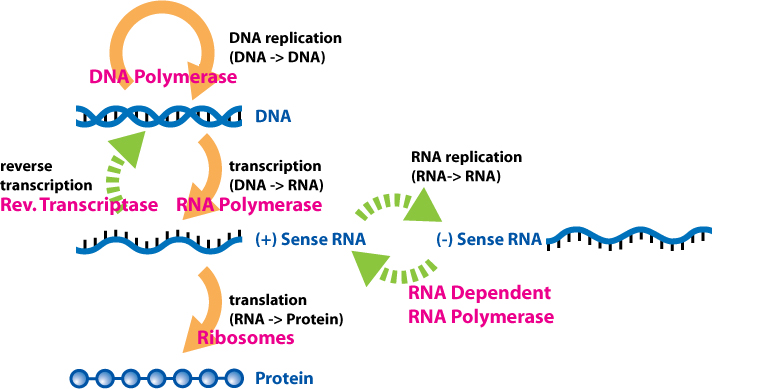
\includegraphics[scale=0.45]{img/dogma.png}
			\caption{\tiny{Fonte: https://en.wikipedia.org/wiki/Central\_dogma\_of\_molecular\_biology}}
		\end{figure}
		\end{frame}

		\begin{frame} \frametitle{Dogma}
		\begin{figure}[hbtp]
			\centering
			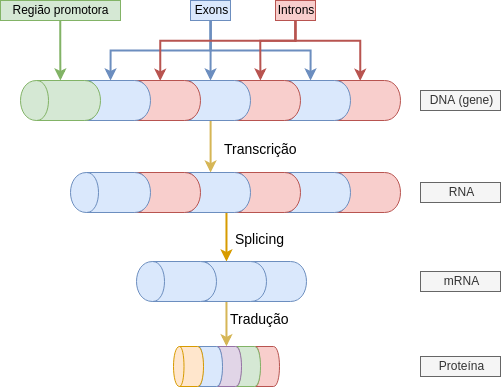
\includegraphics[scale=0.5]{img/dogma_tt.png}
		\end{figure}
		\end{frame}
		
		\begin{frame} \frametitle{DNA}
		\begin{figure}[hbtp]
			\centering
			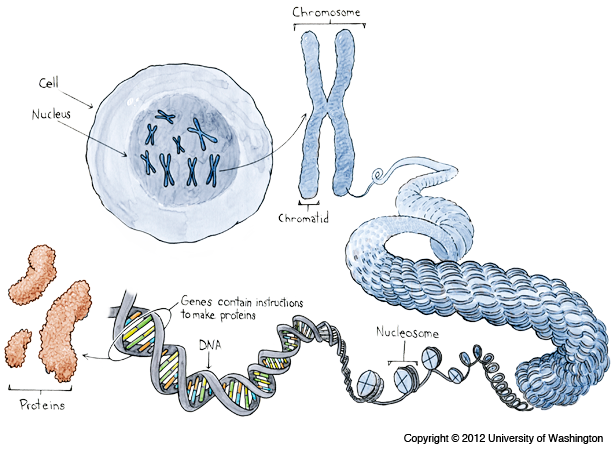
\includegraphics[scale=0.42]{img/dna01.png}
			\caption{\tiny{Fonte: https://www.my46.org/intro/what-is-dna}}
		\end{figure}
		\end{frame}	
	
		\begin{frame} \frametitle{DNA}
		\begin{figure}[hbtp]
			\centering
			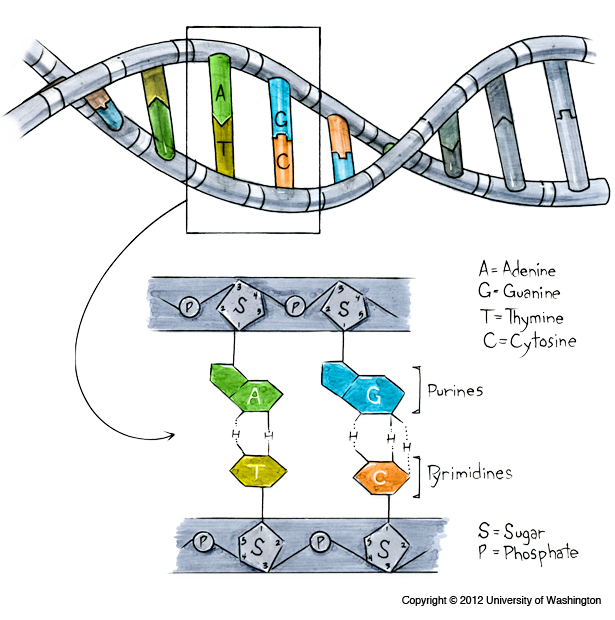
\includegraphics[scale=0.3]{img/dna02.png}
			\caption{\tiny{Fonte: https://www.my46.org/intro/what-is-dna}}
		\end{figure}
		\end{frame}	
	
		\begin{frame} \frametitle{DNA}
		\begin{figure}[hbtp]
			\centering
			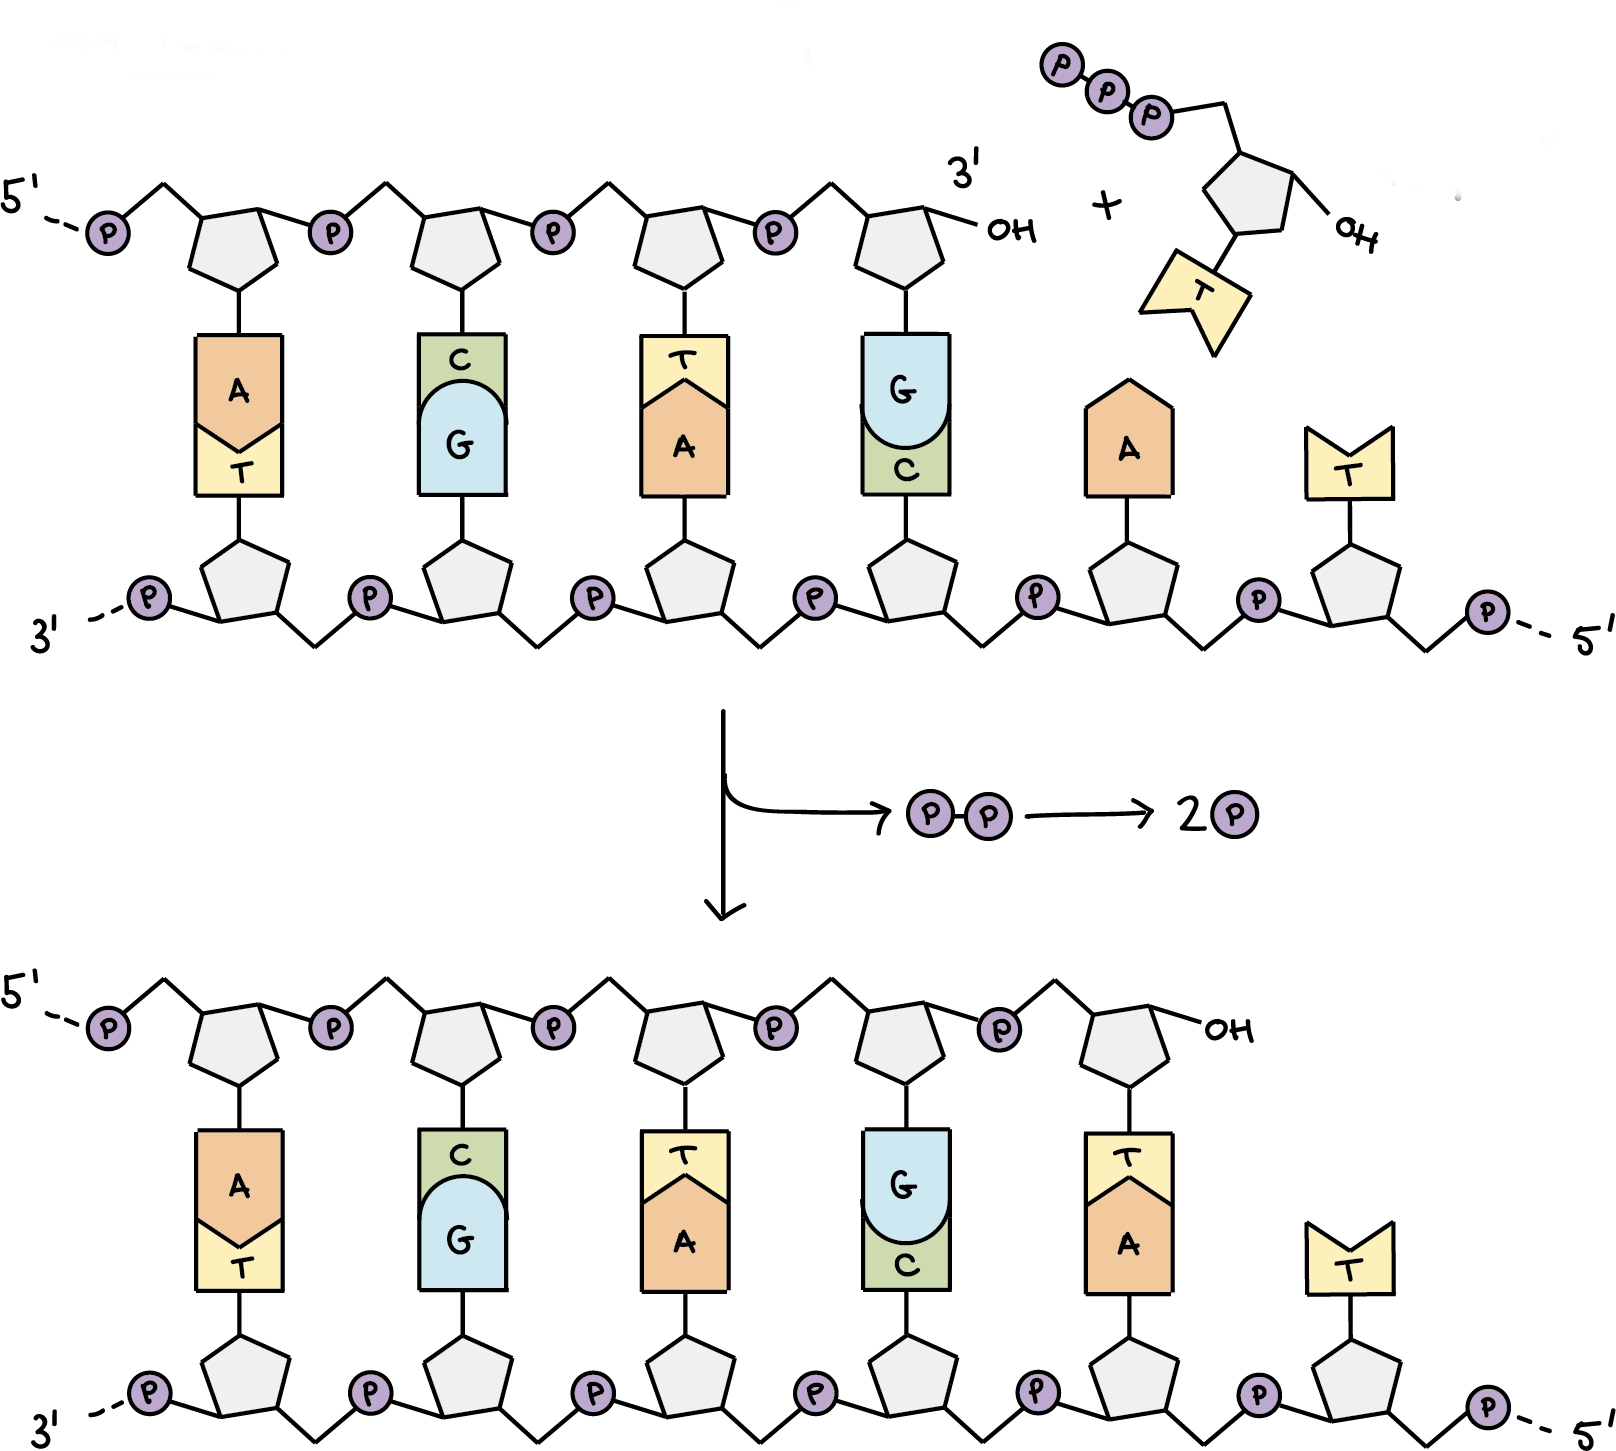
\includegraphics[scale=0.15]{img/dna03.png}
			\caption{\tiny{Fonte: https://www.khanacademy.org}}
		\end{figure}
		\end{frame}		
	
		\begin{frame}\frametitle{Sequenciamento de DNA}
			\begin{itemize}
				\item Obter string(s) representando as moléculas que compõem o DNA
				\item Ainda não é possível sequenciar toda a molécula diretamente
				\item Sequenciar pedaços da molécula, começando em alguma posição na direção 5' $\rightarrow$ 3'
				\item Fragmento (\textit{read}): substring de uma das fitas da molécula alvo
				de DNA
				\item Não sabemos:
				\begin{itemize}
					\item A que fita pertence
					\item A posição relativa ao início da fita
				\end{itemize}
			\end{itemize}
		\end{frame}
		
	%%%%%%%%%%%%%%%%%%%%%%%%%%%%%%%%%%%%%%%%%%%%%%%%%%%%%%%%%%%%%%%%%%%%%%%%%%%%%%%%%%%%%%%%%
	\section{Comparação de sequências}
		\begin{frame}\frametitle{Alinhamento}
			Posicionamento das sequências, preservando a ordem dos nucleotídeos ou aminoácidos e indicando as posições em que as sequências são iguais ou diferentes
			\begin{itemize}
				\item Ferramenta básica da Bioinformática
				\item Alfabeto
				\begin{itemize}
					\item DNA/RNA - 4 nucleotídeos (ACGT/ACGU)
					\item Proteínas - 20 aminoácidos (A, R, N, D, E, C, G, Q, H, I, L, K, M, F, P, S, Y, T, W, V)
				\end{itemize}
				\item Interesse no alinhamento ótimo: o máximo de similaridade e o mínimo de diferenças			
			\end{itemize}
		\end{frame}
	
		\begin{frame}\frametitle{Alinhamento}
			\begin{itemize}
				\item Identidade $\rightarrow$ Porcentagem de aminoácidos (ou nucleotídeos) com um \textit{match} direto no alinhamento
				\item Similaridade $\rightarrow$ Porcentagem de \textit{matches} idênticos e similares (substituição conservativa)\\
						\textcolor{ExecusharesGrey}{\footnotesize\hspace{1em}Exemplo: arginina $\leftrightarrow$ lisina}
						\begin{figure}[hbtp]
							\centering
							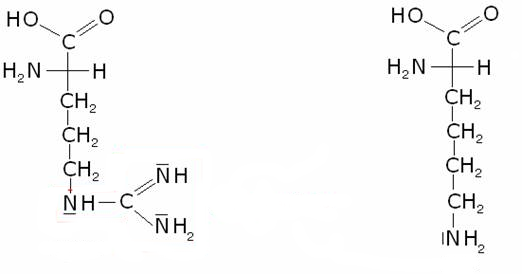
\includegraphics[scale=0.3]{img/arginina_to_lisina.png}
						\end{figure}
				\item Homologia $\rightarrow$ Similaridade entre sequências que dividem ancestral comum
			\end{itemize}
		\end{frame}
		
		\begin{frame}\frametitle{Alinhamento}
		\begin{block}{Exemplo}
			$\linebreak$
			R~O~S~A~V~E~R~M~\textcolor{red}{E}~L~H~A\\
			A~M~O~R~O~S~O~V~\textcolor{red}{E~}R~M~E
			$\linebreak$
			$\linebreak$
			8\% de identidade (1 em 12).
		\end{block}
	    \end{frame}
    
    	\begin{frame}\frametitle{Alinhamento}
    	\begin{block}{Exemplo}
    		$\linebreak$
    		$\ominus$ $\ominus$ $\ominus$ \textcolor{red}{R O S} A \textcolor{red}{~V E R M~E} L ~H ~A\\
    		~A M O \textcolor{red}{~R O S} O \textcolor{red}{V E R M E} $\ominus$ $\ominus$ $\ominus$
    		$\linebreak$
    		$\linebreak$
    		53\% de identidade (8 em 15).
    	\end{block}
	    \end{frame}
    
    	\begin{frame}\frametitle{Alinhamento}
    	\begin{block}{Tipos de alinhamento}\end{block}
    	\begin{block}{Quanto à quantidade de entradas}
    		a) Pairwise - pareamento de 2 sequências\\
    		b) Alinhamento múltiplo - múltiplas sequências
    	\end{block}
    	\begin{block}{Quanto à estratégia de alinhamento}
    		a) Global\\
    		b) Local
    	\end{block}
    	\begin{block}{Quanto ao tipo de entrada}
    		DNA x RNA x Proteína
    	\end{block}
    \end{frame}

	\begin{frame}\frametitle{Alinhamento}
	\begin{block}{Erros}
		\begin{figure}[hbtp]
			\centering
			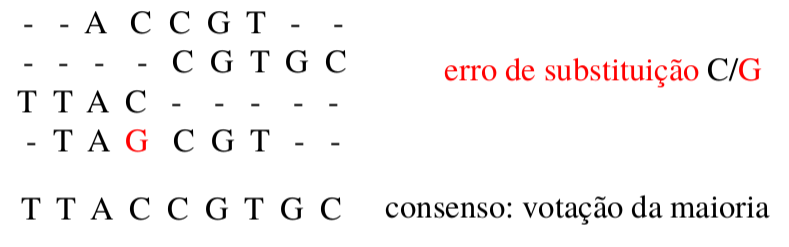
\includegraphics[scale=0.4]{img/erroSubstituicao.png}
		\end{figure}
	\end{block}
	\end{frame}
	%%%%%%%%%%%%%%%%
	\begin{frame}\frametitle{Alinhamento de sequências}
	\begin{block}{Erros}
	\begin{figure}[hbtp]
		\centering
		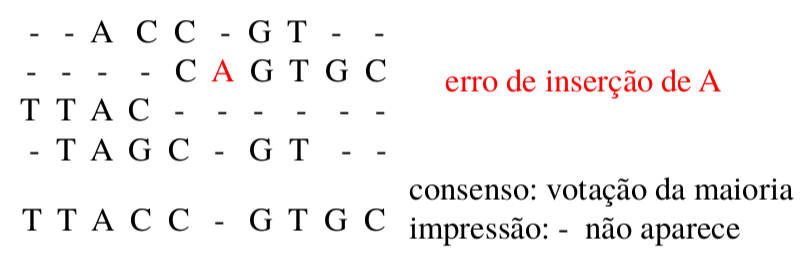
\includegraphics[scale=0.4]{img/erroInsercao.png}
	\end{figure}
	\end{block}
	\end{frame}
	%%%%%%%%%%%%%%%%
	\begin{frame}\frametitle{Alinhamento de sequências}
	\begin{block}{Erros}
	\begin{figure}[hbtp]
	\centering
	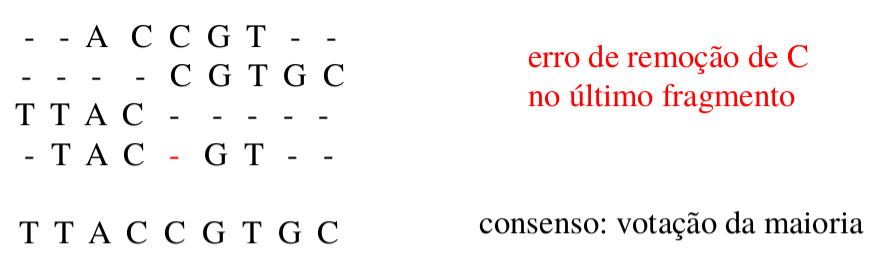
\includegraphics[scale=0.37]{img/erroRemocao.png}
	\end{figure}
	\end{block}
	\end{frame}
	\begin{frame}\frametitle{Alinhamento de sequências}
	\begin{block}{Modelos de pontuação}
		\begin{itemize}
			\item Substituições
			\item Gaps (inserções/deleções)
			\item Matriz de substituição
		\end{itemize}
	\end{block}
	\end{frame}
	%%%%%%%%%%%%%%%%
	\begin{frame}\frametitle{Alinhamento}
	\begin{block}{Modelos de pontuação}
	\begin{itemize}
		\item Tomando as sequências: GACGGATTAG e GATCGGAATAG
		\item \textit{Match} = +1
		\item \textit{Mismatch} = -1
		\item \textit{Gap} = -2
		\begin{table}
			\begin{tabular}{ccccccccccc}
				G  & A  & -  & C  & G  & G  & A  & T  & T  & A  & G  \\
				G  & A  & T  & C  & G  & G  & A  & A  & T  & A  & G  \\ \hline
				+1 & +1 & -2 & +1 & +1 & +1 & +1 & -1 & +1 & +1 & +1 \\
			\end{tabular}
		\end{table}
		\item Obs: Valores das penalidades podem ser escolhidos
	\end{itemize}
	\end{block}
	\end{frame}

	\begin{frame}\frametitle{Alinhamento}
	\begin{block}{Pairwise}
		\begin{itemize}
			\item Alinhamento global (algoritmo de Needleman-Wunsch)
			\item Alinhamento local - \textit{substrings} - (algoritmo de Smith-Waterman)
			\item Alinhamento semi-global - \textit{alinhar prefixos e sufixos}
		\end{itemize}
	\end{block}
	\end{frame}


	\begin{frame}\frametitle{Alinhamento}
	\begin{block}{Alinhamento global}\end{block}
	\begin{figure}[hbtp]
		\centering
		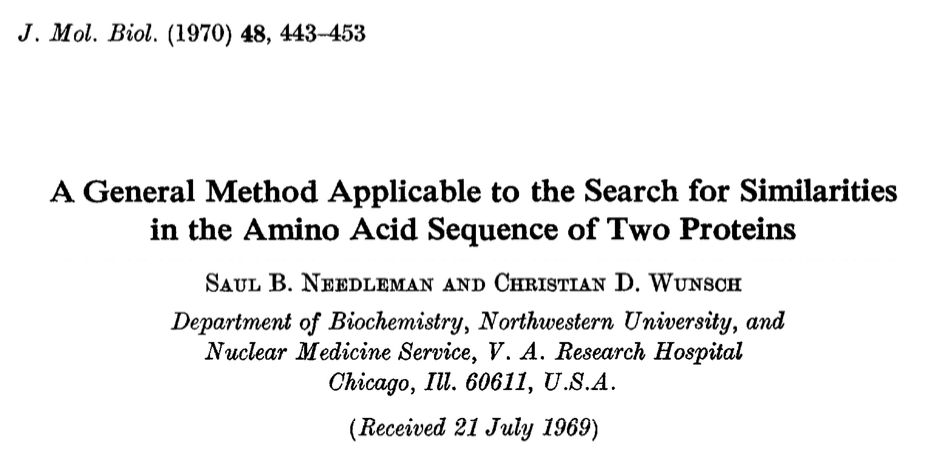
\includegraphics[scale=0.3]{img/needleman.png}
	\end{figure}
	\end{frame}

	\begin{frame}\frametitle{Alinhamento}
	\begin{block}{Alinhamento local}
		\begin{figure}[hbtp]
			\centering
			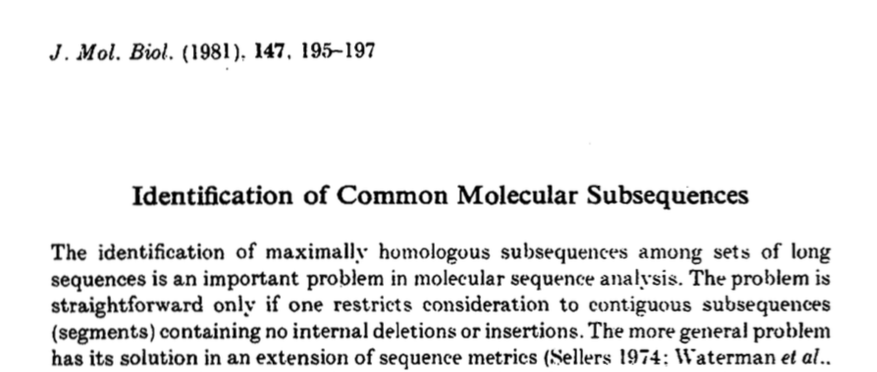
\includegraphics[scale=0.35]{img/smith_waterman.png}
		\end{figure}
	\end{block}
	\end{frame}

	\begin{frame}\frametitle{Alinhamento}
		\begin{figure}[hbtp]
			\centering
			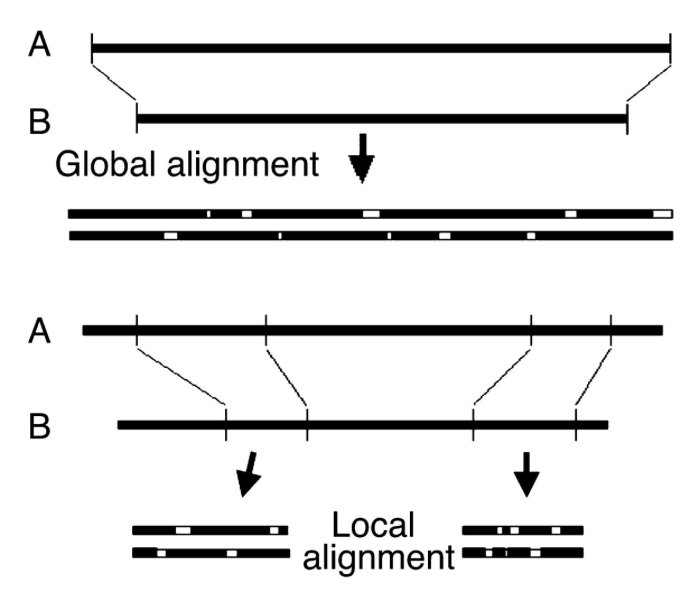
\includegraphics[scale=0.28]{img/global_local.png}
			\caption{Penacchio et al. 2003}
		\end{figure}
	\end{frame}

	\begin{frame}\frametitle{Alinhamento}
		\begin{block}{Matrizes de susbstituição}
		
		\begin{minipage}{\textwidth}
			\begin{minipage}[ht]{0.49\textwidth}
				\begin{figure}[ht]
					\centering
					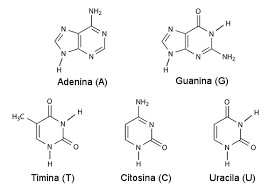
\includegraphics[scale=0.5]{img/pu_py.png}
				\end{figure}
			\end{minipage}
			\hfill
			\begin{minipage}[ht]{0.49\textwidth}
				\centering
				\begin{tabular}{c|c|c|c|c}
					~ & A  & C  & G  & T  \\ \hline
					A & +20 & +5  & +10 & +5  \\ \hline
					C & +5  & +20 & +5  & +10 \\ \hline
					G & +10 & +5  & +20 & +5  \\ \hline
					T & +5  & +20 & +5  & +10 \\
				\end{tabular}
			\end{minipage}
		\end{minipage}
		\end{block}
	\end{frame}
	
	\begin{frame}\frametitle{Alinhamento}
	\begin{block}{PAM (Percent Accepted Mutation) (Dayhoff et al., 1972)}
		\begin{itemize}
			\item Baseada em alinhamento global de proteínas relacionadas alinhadas sem gaps ()mutações são muito significantes)
			\item Probabilidadede um aminoácido ser substituído por outro (eventos independentes HMM)
			\item PAM1: 1\% de mutações aceitas ou seja as sequências tem 99\% de similaridade (aminoácidos idênticos)
			\item PAM250: PAM1 x PAM1, 250 vezes - representando milhões de anos de evolução: melhor para sequências menos relacionadas
		\end{itemize}
	\end{block}
	\end{frame}
	
	\begin{frame}\frametitle{Alinhamento}
	$\linebreak$
	\begin{block}{BLOSUM (BLOck SUbstitution Matrices) (Henikoff \& Henikoff, 1992)}		
		\begin{figure}[hbtp]
			\centering
			
\includegraphics[scale=0.28]{img/blosum62.png}
			\caption{\tiny{BLOSUM62: sequências com mais de 62\% de identidade.}}
		\end{figure}
	\end{block}
	\end{frame}

	\begin{frame}\frametitle{Alinhamento}
	\begin{block}{Blast}
		\begin{itemize}
			\item Basic Local Alignment Search Tool (Altschul \textit{et al.}, 1990)
				\begin{itemize}
					\item Abordagem heurística
					\item Acha palavras curtas e monta tabela hash
					\item Procura palavras curtas em um banco de dados e estende-as quando há um HSP (\textit{High Scoring Segment Pair})
					\item Calcula estatística do alinhamento e interrompe-o quando o \textit{e-value} torna-se menor do que um determinado limite
				\end{itemize}
		\end{itemize}
	\end{block}
	\end{frame}

	%%%%%%%%%%%%%%%%%%%%%%%%%%%%%%%%%%%%%%%%%%%%%%%%%%%%%%%%%%%%%%%%%%%%%%%%%%%%%%%%%%%%%%%%%
	\section{Dados de sequenciamento de alto desempenho}
	
	\begin{frame}\frametitle{Formatos (FASTQ)}
		\begin{figure}[ht]
			\centering
			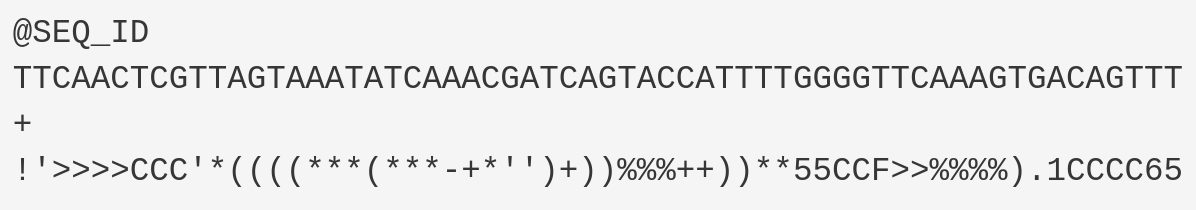
\includegraphics[width=\textwidth]{img/fastq.png}
		\end{figure}
			Exemplo Illumina: \textbf{@HWUSI-EAS100R:6:73:941:1973\#0/1}
			\begin{itemize}
				\item HSWUSI-EAS100R $\rightarrow$ Unique instrument name
				\item 6 $\rightarrow$ Flowcell lane
				\item 73 $\rightarrow$ Tile number within the flow cell lane
				\item 941 $\rightarrow$ x-coordinate of the cluster within the tile
				\item 1973 $\rightarrow$ y-coordinate of cluster within the tile
				\item \#0 $\rightarrow$ Index number for multiplexed sample
				\item /1 $\rightarrow$ Member of a pair
			\end{itemize}
	\end{frame}
	
	\begin{frame}\frametitle{Formatos (FASTQ)}		
		A qualidade (varia de 33 a 126) de cada nucleotídeo sequenciado é representado pelo caractere correspondente da tabela \href{https://upload.wikimedia.org/wikipedia/commons/1/1b/ASCII-Table-wide.svg}{ASCII}.
		
		Os valores \textit{shifted down} para 0 a 93 por compatibilidade com a escala PHRED de qualidade (0 a 60)		
		\begin{figure}[ht]
			\centering
			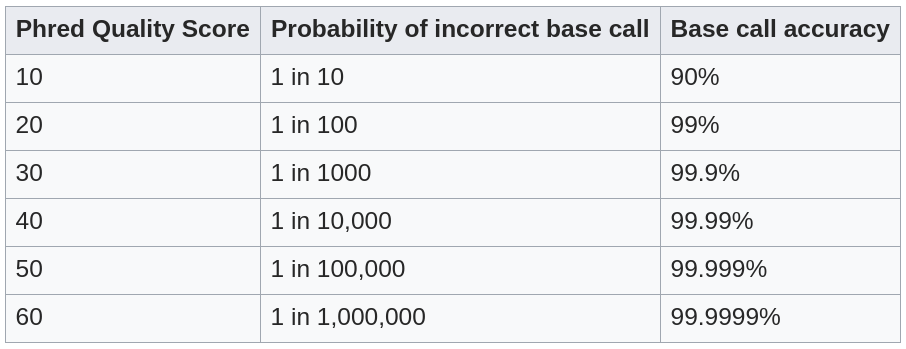
\includegraphics[scale=0.3]{img/phred.png}
		\end{figure}
	\end{frame}

	\begin{frame}\frametitle{Formatos (FASTQ)}
		\begin{figure}[ht]
		\centering
		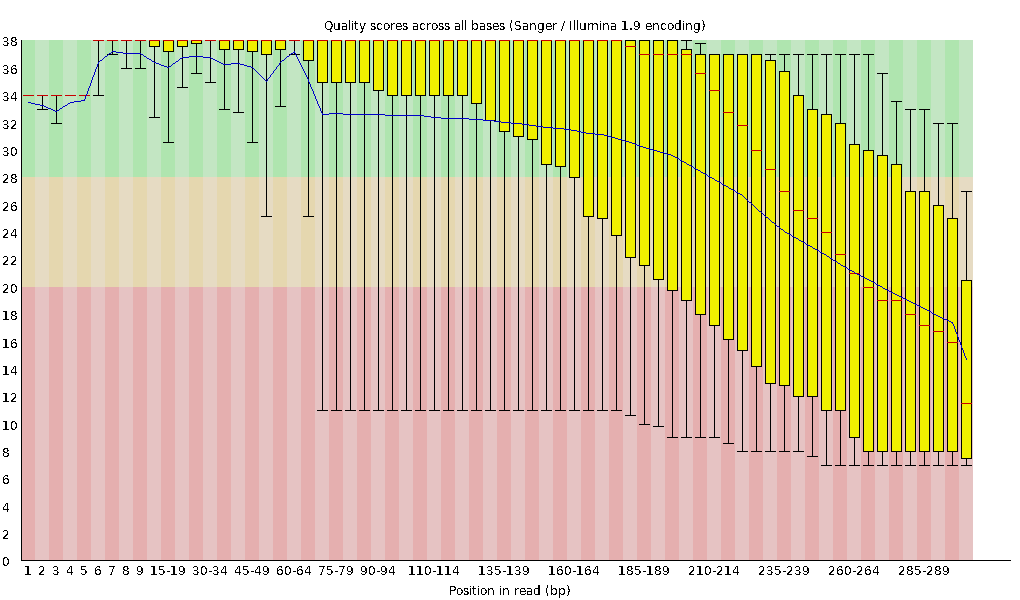
\includegraphics[width=\textwidth]{img/antes}
		\end{figure}
	\end{frame}
%	%%%%%%%%%%%%%%%
	\begin{frame}\frametitle{Formatos (FASTA)}
		\begin{figure}[ht]
		\centering
		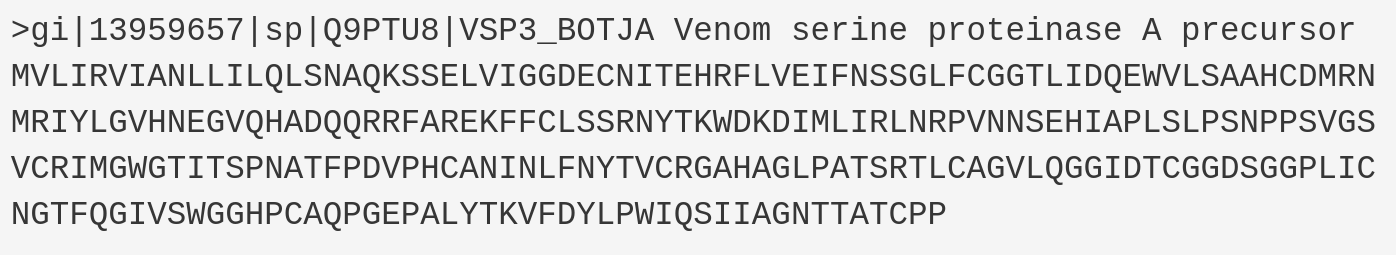
\includegraphics[width=\textwidth]{img/fasta.png}
		\end{figure}
		\begin{tiny}
		\begin{enumerate}
		\item Cabeçalho
		\begin{itemize}
			\item GenBank/EMBL $\rightarrow$ gi|gi\_number|*|accession.version|locus
			\item NCBI refseq $\rightarrow$ ref|accession|locus
			\item PRF Protein Research Foundation $\rightarrow$	pir|entry
			\item SWISS-PROT $\rightarrow$ sp|accesion|locus
			\item PDB Protein Data Bank $\rightarrow$ pdb|entry|chain
		\end{itemize}
		\item Sequência
		\begin{itemize}
			\item nucleotídeos ou aminoácidos
		\end{itemize}
		\end{enumerate}
		\end{tiny}
	\end{frame}


	\begin{frame}\frametitle{Formatos (FASTA)}
		\begin{itemize}
		\item .fasta, .fa $\rightarrow$ arquivo fasta genérico 
		\item .fna $\rightarrow$ FASTA nucleotídeos
		\item .ffn $\rightarrow$ FASTA regiões codificadoras (nucleotídeos)
		\item .faa $\rightarrow$ FASTA aminoácidos
		\item .frn $\rightarrow$ FASTA RNA não codificador
		\end{itemize}
		\begin{itemize}
		\item Multi-fasta $\rightarrow$ múltiplas sequências em um único arquivo
		\end{itemize}
	\end{frame}

	\begin{frame}\frametitle{Formatos (SAM, BAM)}
		\href{http://www.htslib.org/}{SAMTools} fazem pós-processamento de alinhamentos de \textit{reads}, as quais são sequências de DNA em formato FASTQ.\\
		\begin{itemize}
		\item SAM (Sequence Alignment/MAP) guarda o alinhamento das \textit{reads} e pode ser lido por diversos softwares como o IGV (Integrated Genome Viewer).
		\item BAM (Binary Alignment/MAP) é uma versão comprimida de um alinhamento das \textit{reads}. Pode ser obtido diretamente do alinhamento ou convertido a partir de um arquivo SAM.
		\end{itemize}
	\end{frame}

	\begin{frame}\frametitle{Formatos (SAM, BAM)}
	\begin{figure}[ht]
		\centering
		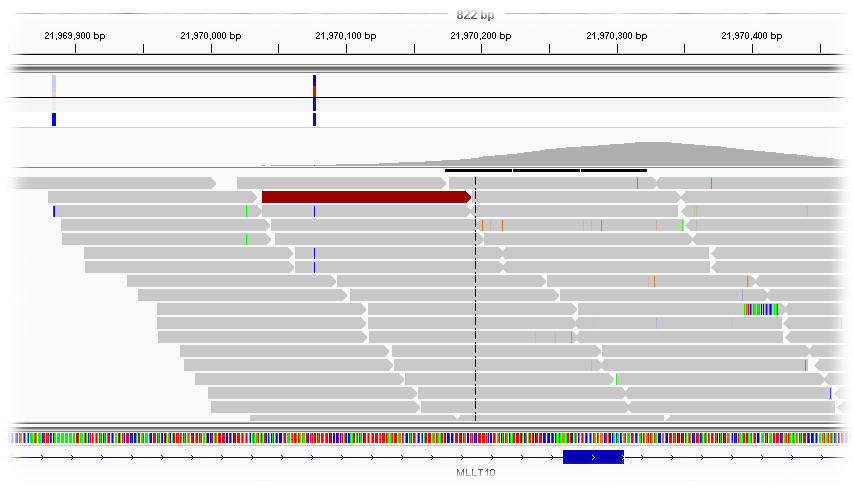
\includegraphics[width=\textwidth]{img/igv.png}
	\end{figure}
	\end{frame}


	\begin{frame}\frametitle{Formatos (BED)}
		\begin{itemize}
		\item BED é um arquivo organizado em colunas separadas por tabulação (tab) com anotações da sequência
		\item Pode ser aberto em um genome browser
		\end{itemize}
		\begin{figure}[ht]
		\centering
		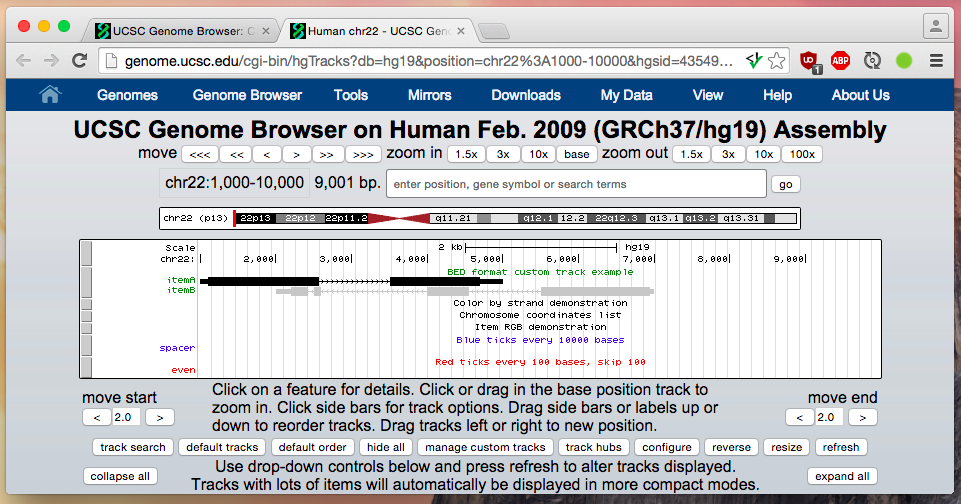
\includegraphics[scale=0.25]{img/bed.png}
		\end{figure}
	\end{frame}
%
%
	\begin{frame}\frametitle{Formatos (BED)}
		\begin{itemize}
		\item Arquivos BED têm 12 colunas, 1-3 obrigatórias, 4-12 opcionais
		\begin{enumerate}
		\item \textbf{chrom} $\rightarrow$ nome do cromossomo no qual a \textit{feature} existe
		\item \textbf{start} $\rightarrow$ posição inicial na sequência
		\item \textbf{end} $\rightarrow$ posição final na sequência
		\item name $\rightarrow$ nome da \textit{feature}
		\item score $\rightarrow$ 0 and 1000 (nível de cinza$^1$)
		\item strand $\rightarrow$ direção da fita ``+'' ou ``-''
		\item thickStart $\rightarrow$ posição inicial onde a \textit{feature} é desenhada
		\item thickEnd $\rightarrow$ posição final onde a \textit{feature} é desenhada
		\item itemRgb $\rightarrow$ determina a cor dos dados
		\item blockCount $\rightarrow$ número de bloco (exons)
		\item blockSizes $\rightarrow$ lista de blocos separados por vírgula
		\item blockStarts $\rightarrow$ lista de posições iniciais dos blocos
		\end{enumerate}
		\end{itemize}
		\tiny{1) Pode ser usado para outras medidas como p-value, up/down, ...}
	\end{frame}


	\begin{frame}\frametitle{Formatos (GFF)}
		\begin{itemize}
		\item GFF são similares aos BED e têm 9 colunas obrigatórias
		\begin{enumerate}
		\item seqname $\rightarrow$ nome da sequência
		\item source $\rightarrow$ origem da \textit{feature}
		\item feature $\rightarrow$ tipo de \textit{feature}, equivalente ao campo \textit{name} do BED
		\item start $\rightarrow$ posição inicial
		\item end $\rightarrow$ posição final
		\item score $\rightarrow$ assim como o arquivo BED permite níveis de valores representando a expressividade da anotação
		\item strand $\rightarrow$ direção da fita ``+'' ou ``-''
		\item frame $\rightarrow$ frame da sequência codificadora: ``0'',``1'',``2'' ou ``.'',
		\item attribute $\rightarrow$ muda conforme a versão do GFF (GFF1, GFF2, GFF3) e denota texto livre com algum significado biológico
		\end{enumerate}
		\end{itemize}
	\end{frame}

	\section{Filtragem e montagem de fragmentos}
	
		\begin{frame}\frametitle{Filtragem}
		\begin{figure}[ht]
			\centering
			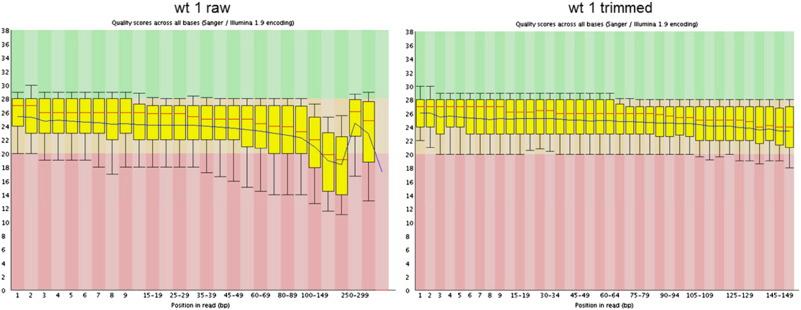
\includegraphics[scale=0.6]{img/filtragem.png}
			\caption{\tiny{\href{http://dx.doi.org/10.1016/j.gdata.2015.05.013}{RNA-Seq analysis of isolated satellite cells in Prmt5 deficient mice}}}
		\end{figure}
		\end{frame}
	
		\begin{frame}\frametitle{Montagem (Grafo De Brujin)}
		\begin{figure}[ht]
			\centering
			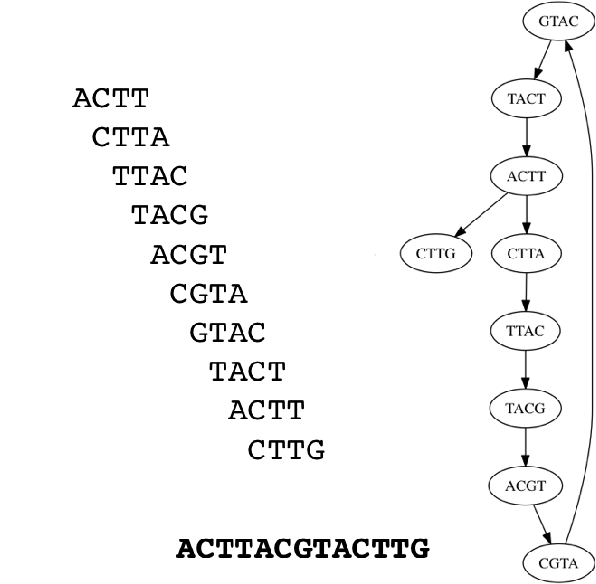
\includegraphics[width=.6\textwidth]{img/dbrujin.png}
		\end{figure}
		\end{frame}
	
		\begin{frame}\frametitle{Montagem (Grafo De Brujin)}
		\begin{itemize}
			\item Um caminho \textit{Euleriano} visita cada aresta exatamente uma vez
			\item Existe um caminho Euleriano se, e somente se:
			\begin{enumerate}
				\item máximo de 2 nós semi-balanceados
				\item todos os demais nós são balanceados
			\end{enumerate}
			\item Um nó é balanceado se \textit{indegree} e \textit{outdegree} são iguais
			\item Um nó é semi-balanceado se a diferença máxima de \textit{indegree} e \textit{outdegree} é 1
			\item um grafo é conectado se cada nó pode ser alcançado por algum outro nó		
		\end{itemize}
		\end{frame}
	
		\begin{frame}\frametitle{Montagem (Grafo De Brujin)}
			\textbf{k-mer} é uma substring de tamanho \textbf{k}\\
			Exemplo: Seja a String \textcolor{blue}{GGCGATTCATCG}, então todos os 3-mer:
			\begin{figure}[ht]
				\centering
				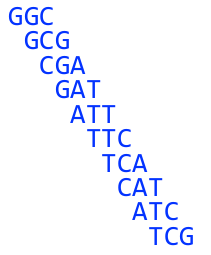
\includegraphics[width=.34\textwidth]{img/3-mer.png}
			\end{figure}
		\end{frame}
	
		\begin{frame}\frametitle{Montagem (Grafo De Brujin)}
		\begin{figure}[ht]
			\centering
			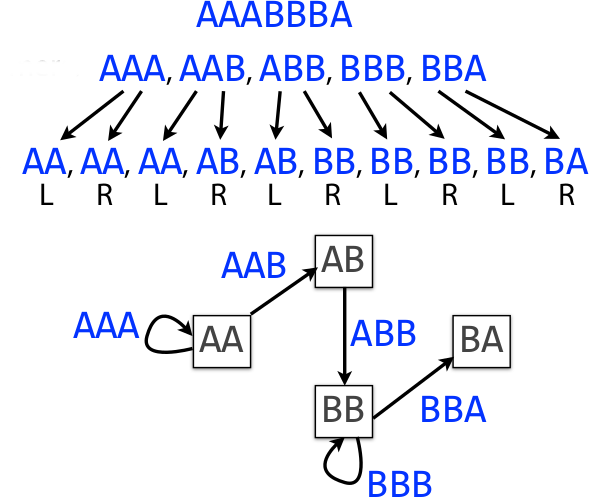
\includegraphics[width=.75\textwidth]{img/debrujinresume.png}
		\end{figure}
		\end{frame}
	
		\begin{frame}\frametitle{Prática em Laboratório}
		\centering
		\href{https://github.com/waldeyr/bsb2018}{
\includegraphics[scale=0.5]{img/git.png}\\Prática}
		\end{frame}
	
		
\end{document}
